
\section{Bag of Attributes Model\label{sec:boa}}
In this section, we define the proposed FC embedding architecture and the objectives used during training.

\subsection{Architecture}

\begin{figure}
\centering
\subcaptionbox{Self-other attribute encoder for an attribute.\label{fig:self-other}}{
    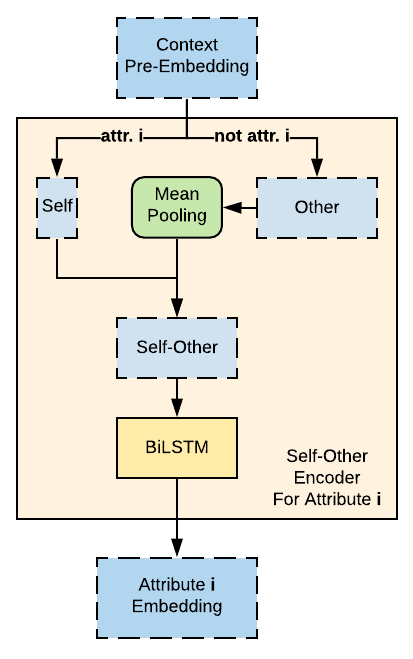
\includegraphics[height=12cm, width=.48\textwidth, keepaspectratio]{Figures/Ch2/boa_self_other_encoder.png}  }
\subcaptionbox{BoA encoder architecture.\label{fig:boa-encoder}}{
    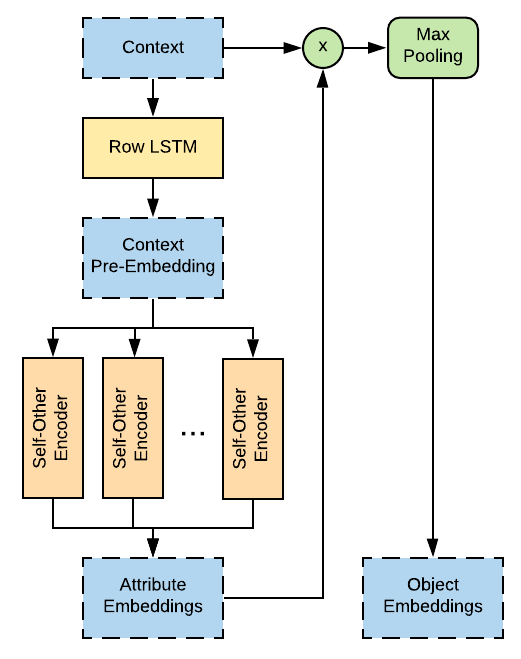
\includegraphics[height=12cm, width=.48\textwidth, keepaspectratio]{Figures/Ch2/boa_encoder.png}  }
\subcaptionbox{BoA decoder architecture.\label{fig:boa-decoder}}{
    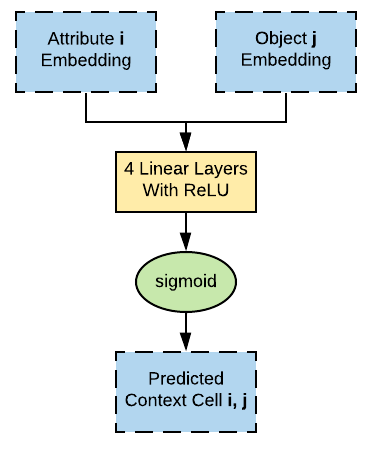
\includegraphics[height=12cm, width=.48\textwidth, keepaspectratio]{Figures/Ch2/boa_decoder.png}  }
\caption{Schematic representation of the BoA architecture. Blue blocks correspond to tensors, the orange to neural components and green blocks to non-neural computations. Arrows joining blocks represent concatenation of tensors.} \label{fig:boa-architecture}
\end{figure}

\textit{Bag of Attributes} (BoA) takes a formal context as input and produces embeddings for its attributes.
Then, object embeddings are computed using the embeddings of the attributes and the formal context.
BoA has four main components: a pre-embedding generator, an attribute encoder called \textit{self-other encoder} to compute the attribute embedding, an object encoder, and a decoder.
The order of the attributes in the FC does not matter for FCA, because intents are unordered sets of attributes.
Therefore, in BoA, the order of the attributes is ignored by design.
BoA considers the attributes as an unordered set to produce the object and attribute embeddings.
The name is an homage to \textit{Bag of Words} (BoW)~\cite{word2vec:2013:mikolov}, which consider sentences as unordered bags of words.

To capture the absence of order between the attributes, they are processed in a similar manner.
Each attribute is compared to all the other attributes, for each object of the FC.
In practice, the column of an attribute (\emph{self}) is compared to an unordered composition (average-pooling) of all the other attributes (\emph{other}).
\emph{Self} and \emph{other} are then concatenated and processed by a BLSTM, with the object dimension as the sequence dimension.
The last hidden state of the BLSTM is processed with a feed-forward layer into an embedding that represents the attribute.
The structure of the attribute encoder is presented in \cref{fig:self-other}.
A $\mu$ and a $\sigma$ vector are produced for each attribute because BoA is trained as a VAE, and the actual embeddings are samples from the normal distributions defined by $\mu$ and $\sigma$.
Finally, the object embeddings are computed by applying max-pooling on the embeddings of the attributes present in the object's intent.
The structure of the encoder is schematized in \cref{fig:boa-encoder}.

%\subsubsection{Pre-Embedding}
This encoder architecture successfully ignores the order of the attributes.
However, we are not able to differentiate between the attributes anymore either, which is a problem to model FCA.
Indeed, we still need to differentiate the attributes to know which ones belong in which intent, even if the order of the attribute does not matter.
Using unordered composition directly on the FC will prevent the model from differentiating, \eg, when an attribute $a_1$ is present and $a_2$ is not from when $a_2$ is present and not $a_1$:
the average of the list $(0, 1)$ is $0.5$, the same as the average of the list $(1, 0)$.
The same kind of problem arises with standard embedding methods using a learned vector to represent each possible value.
In our previous example, if we replace in $C$ every $1$ with the same embedding $emb_1$ and every $0$ by $emb_0$, the model is still unable to determine which one between $a_1$ and $a_2$ is present.
To avoid this issue, we apply an LSTM on each row of $C$ before the \textit{self-other encoder}.
This LSTM can produce different embeddings for each attribute despite the same input, so it allows the model to identify the attributes when the unordered composition is applied.
Indeed, RNNs produce different outputs from the same input if their hidden state is different.

The decoder is an MLP predicting if an object has an attribute or not ($1$ or $0$, respectively).
Its input is the concatenation of the object and the attribute embeddings.
A sigmoid function applied to the output ensures it is in $[0,1]$.
It is schematized in \cref{fig:boa-decoder}.


\subsection{Training Objective}\label{sec:boa-metric}
% We train our BoA model using four objectives.
% %
% The first two are the KL divergence and the reconstruction loss.
% In our case we predict between two classes ($1$ and $0$), so we use the \textit{binary cross entropy} loss for reconstruction.
% The KL divergence is applied on the attribute embeddings exclusively as the sampling happens before the computation of the object embeddings.
We train BoA using KL divergence on the attribute embeddings exclusively because the sampling happens before the computation of the object embeddings.
We use the BCE loss for reconstruction because the model predicts between two classes ($1$ and $0$).
To improve the quality of the embeddings, we use metric learning the \textit{co-intent similarity} (defined in the next paragraph) and the number of concepts~\cite{formal:1999:bernhard}, with \textit{mean square error} (MSE) as the loss function.
We use MLPs to predict the co-intent similarity and number of concepts.
The training setup is schematized in \cref{fig:boa-training}.

\begin{figure}
\centering
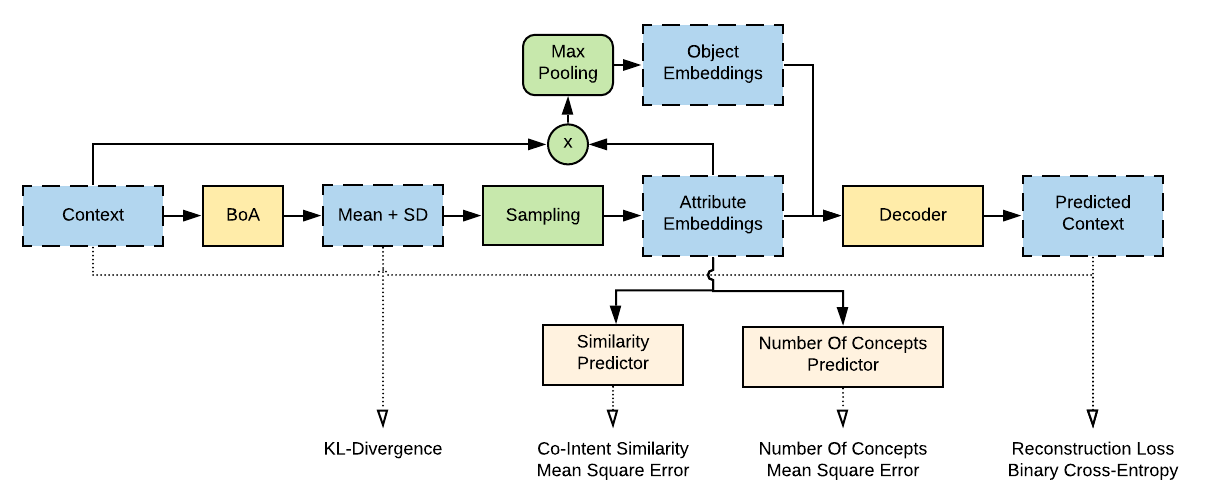
\includegraphics[height=12cm, width=\textwidth, keepaspectratio]{Figures/Ch2/training_flat.png}
\caption{Schematic representation of the BoA architecture training process.} \label{fig:boa-training}
\end{figure}

On the one hand, we need both ``equal'' and ``different'' attributes to use metric learning losses on attribute embeddings.
Nonetheless, even if we consider equivalent attributes (\textit{i.e.} with the same extent) as ``equal'', they are usually rare within a given context.
We define co-intent similarity to compare attributes and avoid this issue.
Given two attributes $a_1$ and $a_2$ we define their \emph{pairwise co-intent similarity} as:
\begin{equation}
\text{co-intent}(a_1, a_2) = 
%
\left\{
    \begin{array}{l}
        1 \text{~~~ if } |\{i\in I| a_1 \in i\}| + |\{i\in I| a_2 \in i\}| = 0 \\\\
        \dfrac{2 \times |\{i\in I| a_1 \in i, a_2 \in i\}|}{|\{i\in I| a_1 \in i\}| + |\{i\in I| a_2 \in i\}|} \text{ otherwise.}
    \end{array}
\right.
\label{equ:co-intent}
\end{equation}
In other words, it is the ratio of intents containing both attributes over the intents containing $a_1$ or $a_2$\footnote{Observe that this is essentially the Jaccard index on the set of intents.}.
In cases where no intent contains the attributes (both attributes are empty or padding columns), the similarity is set to $1$.
Co-intent similarity ranges from $0$, for attributes never appearing in the same intents, to $1$, for attributes always appearing together or for identical attributes.
To predict the co-intent similarity between two attributes $a_1$ and $a_2$, the input of the MLP predictor is the concatenated embeddings of $a_1$ and $a_2$, and a sigmoid output function is added to ensure the predicted similarity is in $[0,1]$.

On the other hand, predicting the number of concepts from the context without actually computing the intents, helps when generating the set of concepts using neural models.
Indeed, knowing how many elements to generate beforehand facilitates the generation process.
Note that counting the number of concepts of a context is \#P-complete (and so, is a ``hard'' task to achieve)~\cite{lattice-size:2001:kuznetsov}.
%\todo{Alain: As a remark, counting the number of concepts of a context is \#P-complete (and so, is a "hard" task to achieve)}
We apply a max-pooling over the attribute embeddings before predicting the number of concepts with the MLP predictor, which corresponds to a \textit{deep averaging network} (DAN)~\cite{dan:2015:iyyer}.

